
\begin{figure}[!h]
  \centering
  \begin{subfigure}{.8\textwidth}
    \centering
    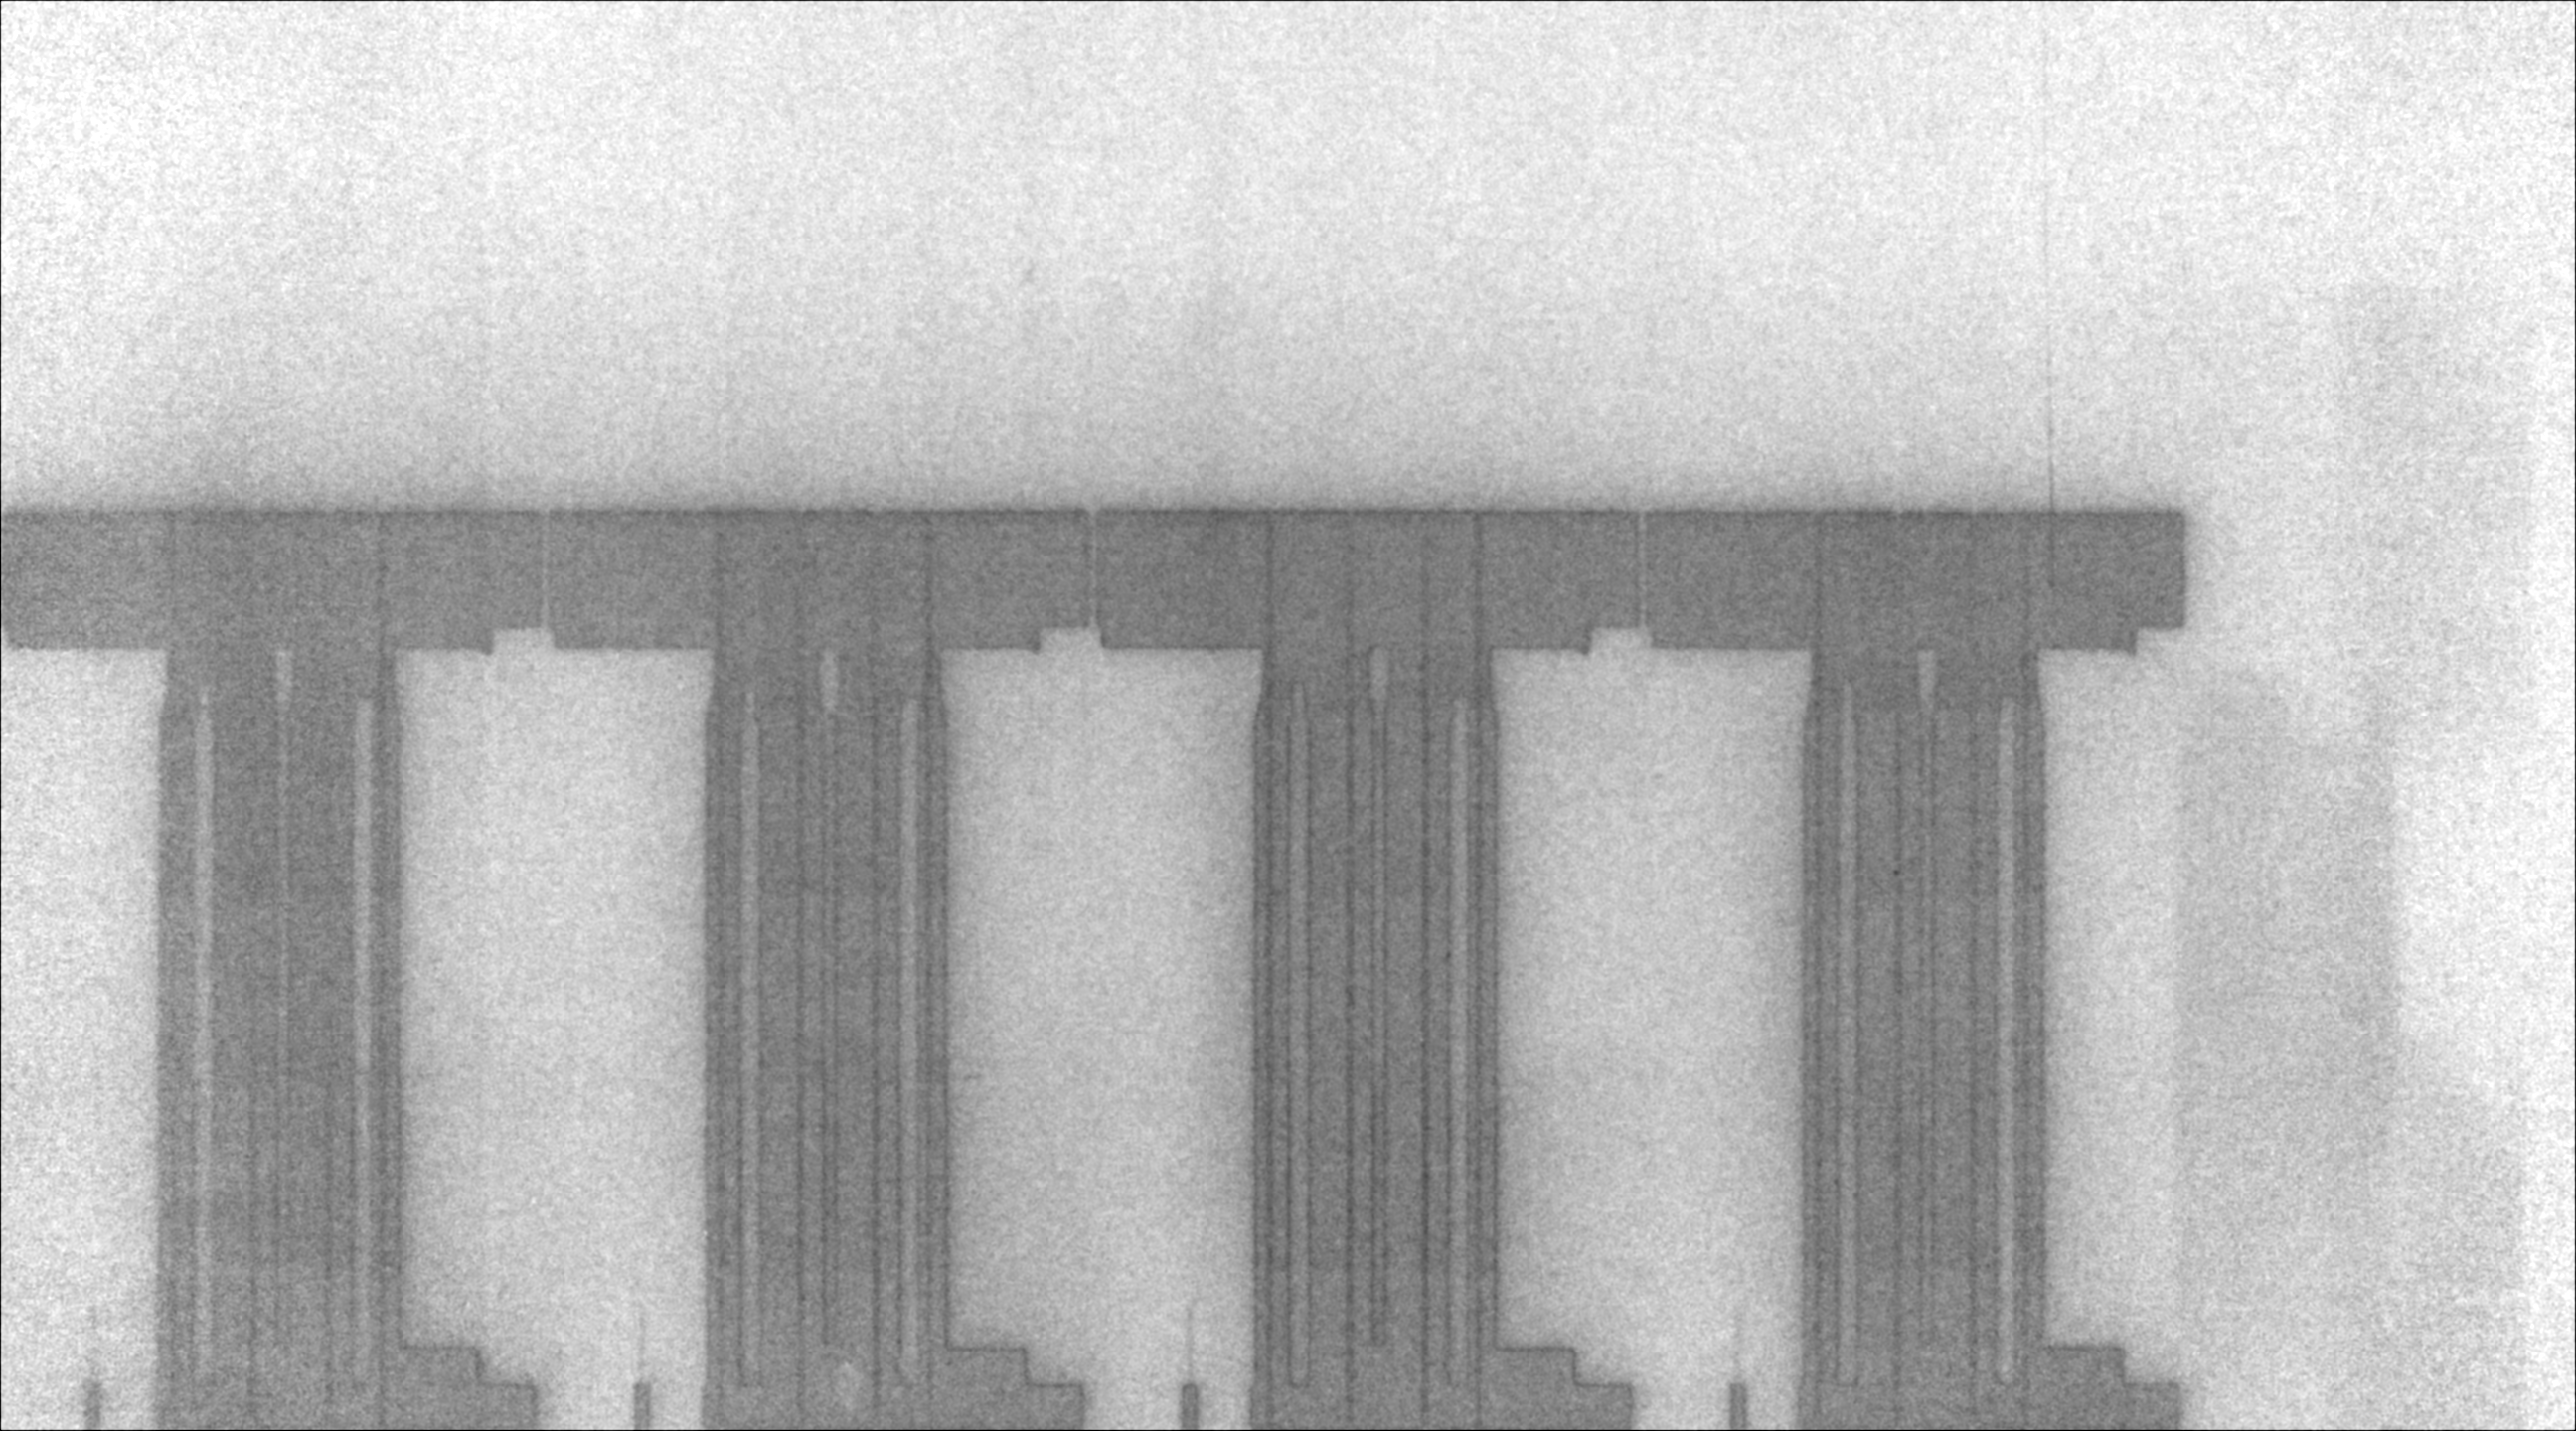
\includegraphics[width=\linewidth]{images/implementation/results/bm/layer_00093}
    \caption{Layer \#93 contains}
  \end{subfigure}

  \begin{subfigure}{.8\textwidth}
    \centering
    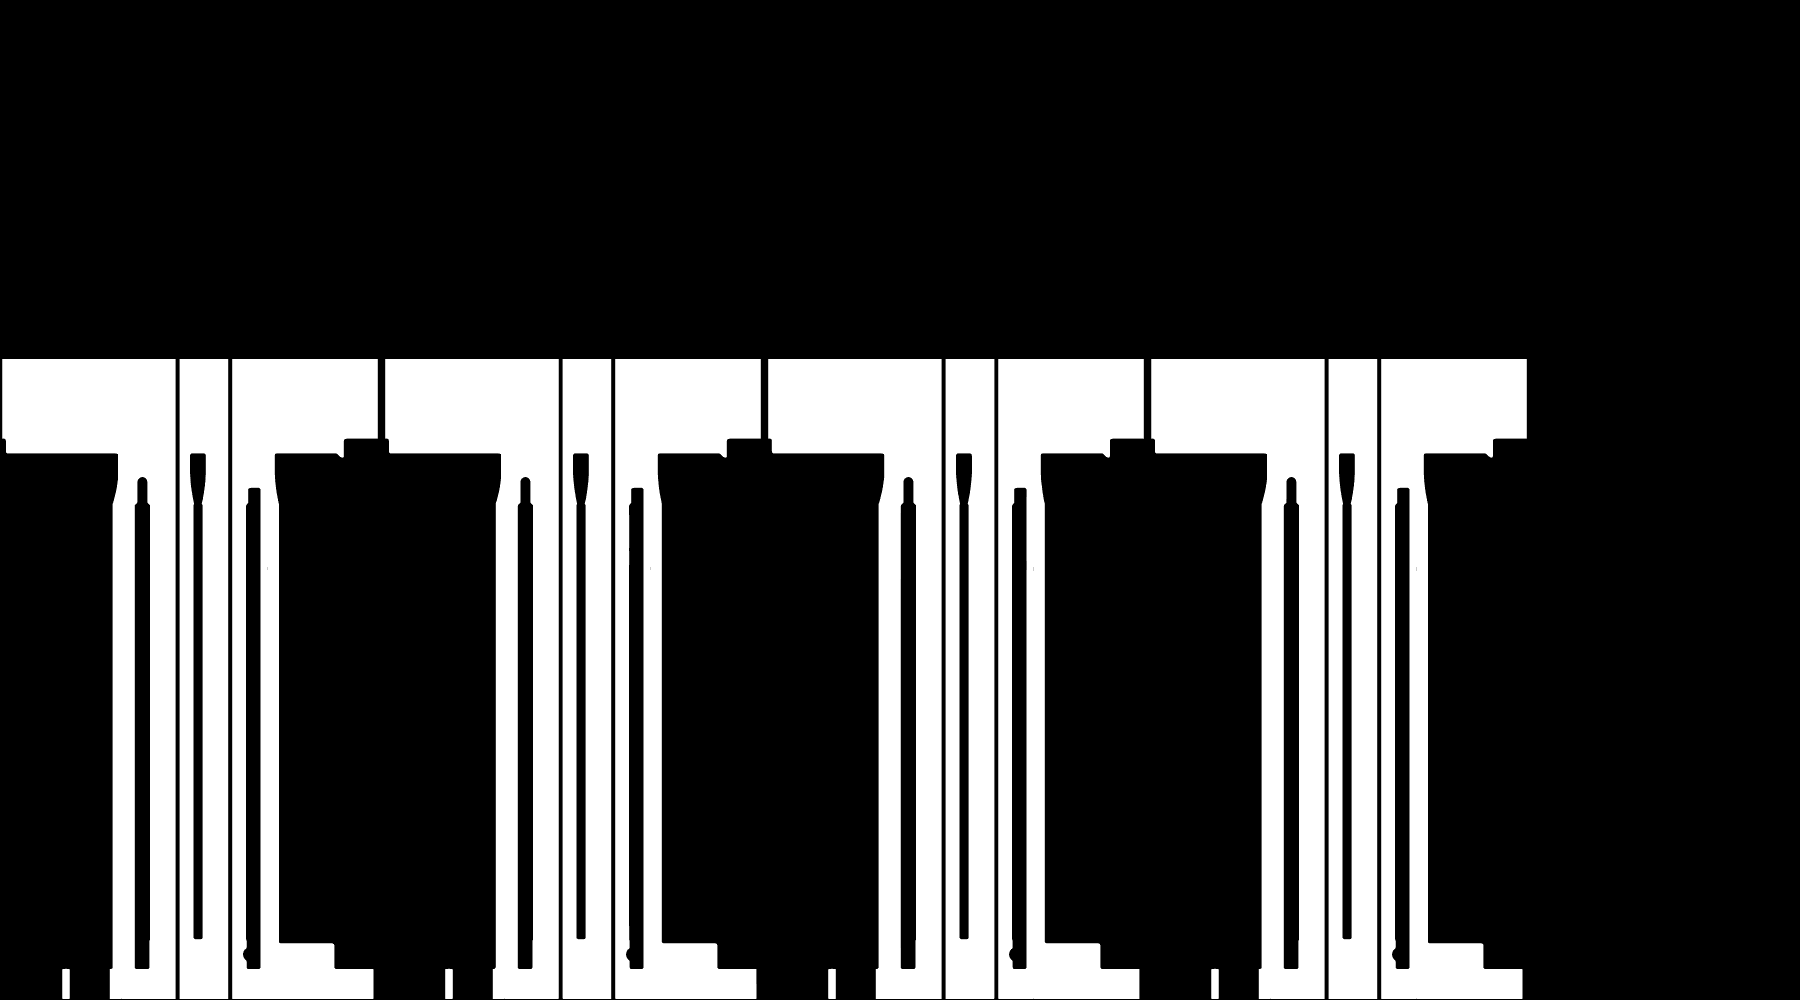
\includegraphics[width=\linewidth]{images/implementation/results/bm/bitmask_00093}
    \caption{Bitmask of layer \#93}
  \end{subfigure}

  \begin{subfigure}{.8\textwidth}
    \centering
    
\includegraphics[width=\linewidth]{images/implementation/results/bm/bitmask_00092}
    \caption{Bitmask of previous layer \#92}
  \end{subfigure}

  \caption{The layer 93 contains closely positioned edges and artifacts from previous. Therefore, this is a good example to highlight different bitmask integration methods. }
  \label{app:layer_example}
\end{figure}

\begin{figure}[!h]
\centering
\begin{subfigure}{.9\textwidth}
  \centering
  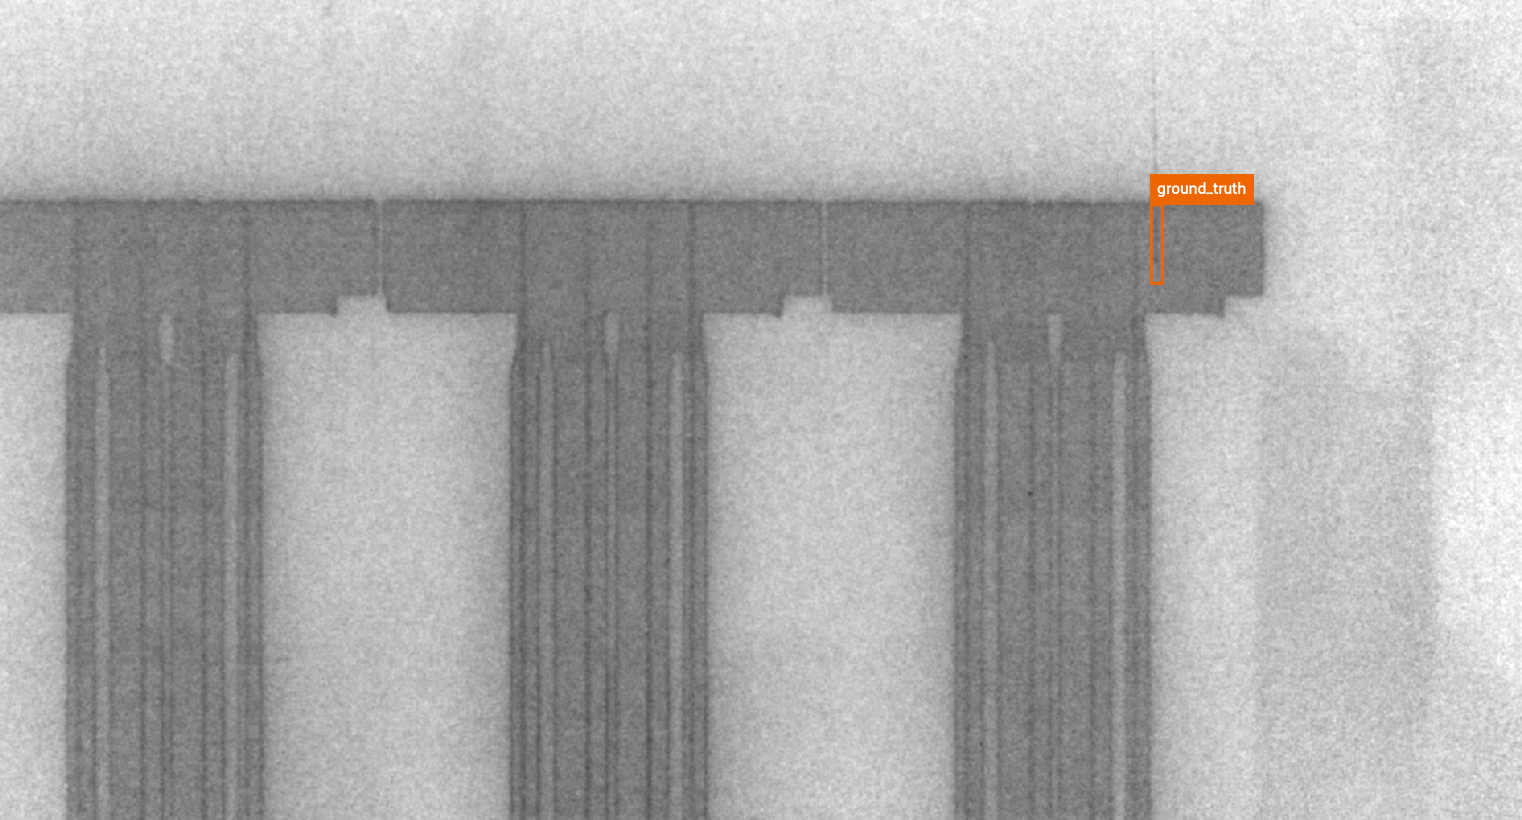
\includegraphics[width=\linewidth]{images/implementation/results/bm/gt}
  \caption{Ground truth}
\end{subfigure}

\begin{subfigure}{.9\textwidth}
  \centering
  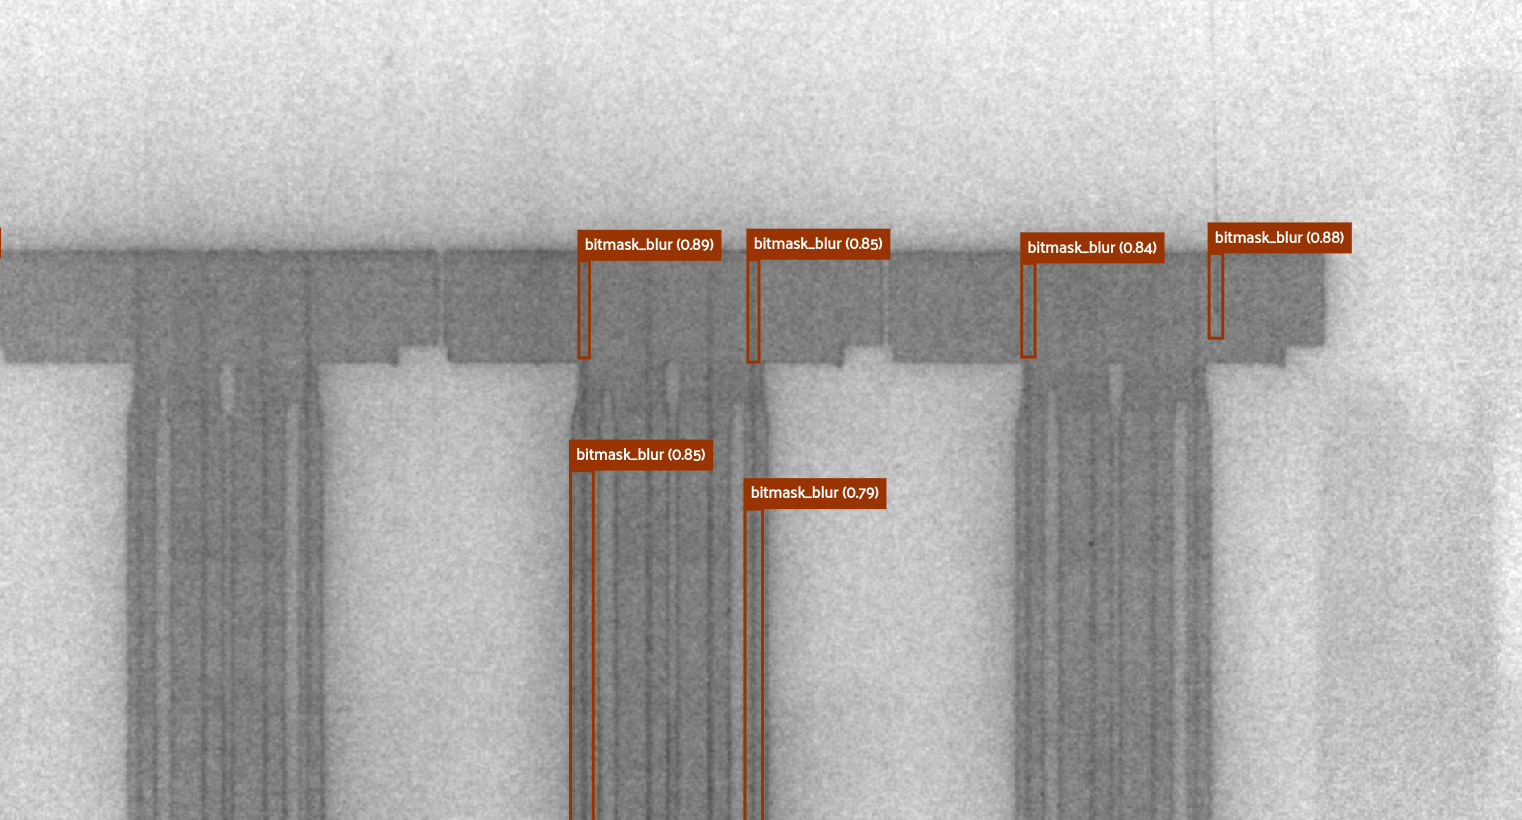
\includegraphics[width=\linewidth]{images/implementation/results/bm/bm_blur}
  \caption{Using a bitmask and it's blurred version}
\end{subfigure}

\begin{subfigure}{.9\textwidth}
  \centering
  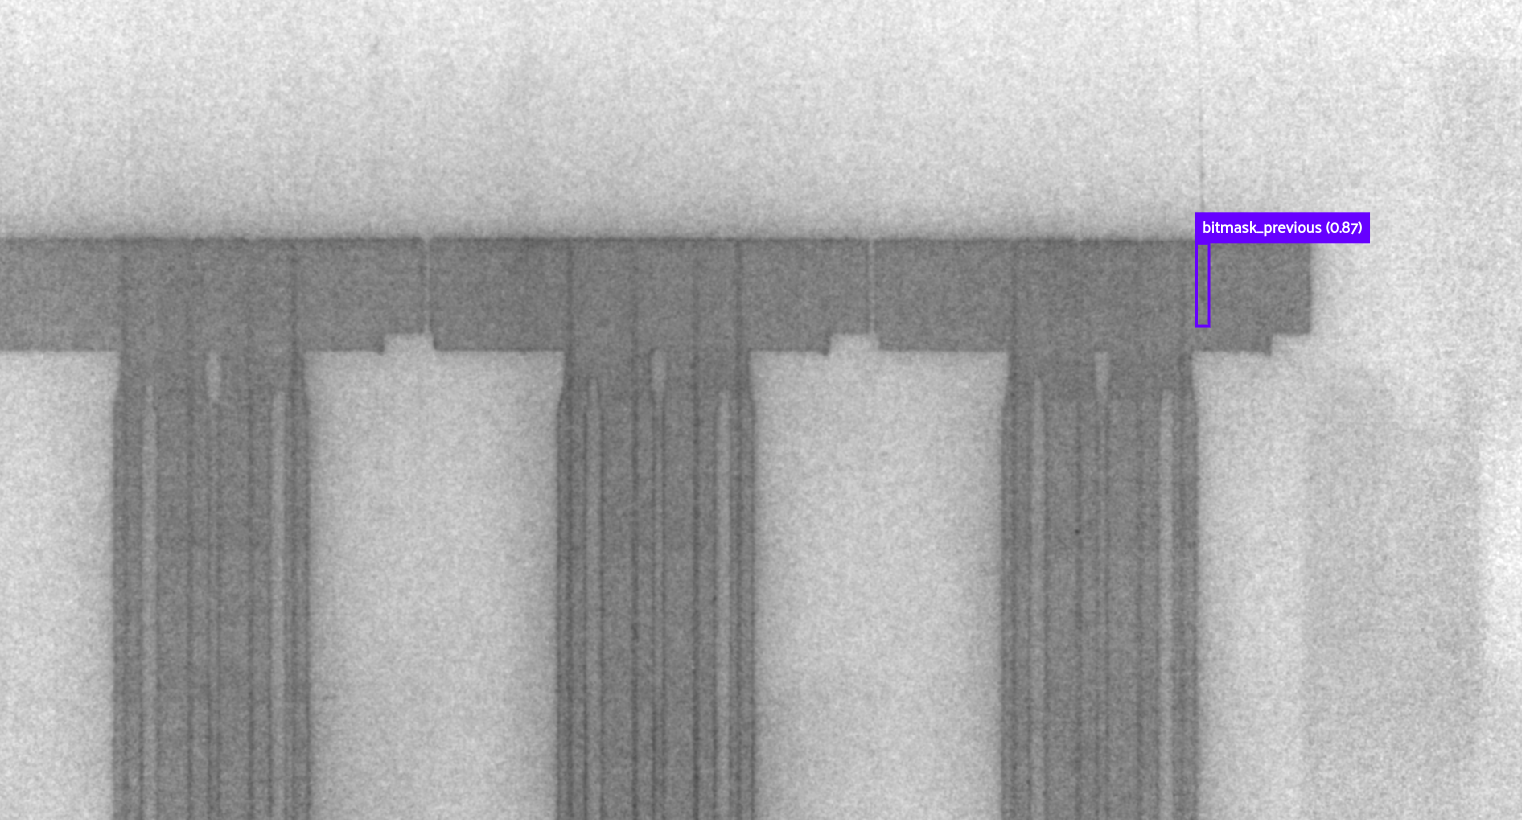
\includegraphics[width=\linewidth]{images/implementation/results/bm/bm_prev}
  \caption{Using current and previous bitmasks}
\end{subfigure}
\caption{The alternative methods tend to have many false positives. The best method that uses the current bitmask and previous bitmask and is therefore able to avoid the false detections. More examples in the appendix.}
\label{app:bm_compare_ext_1}
\end{figure}


\begin{figure}[!h]
\centering

  \begin{subfigure}{.9\textwidth}
    \centering
    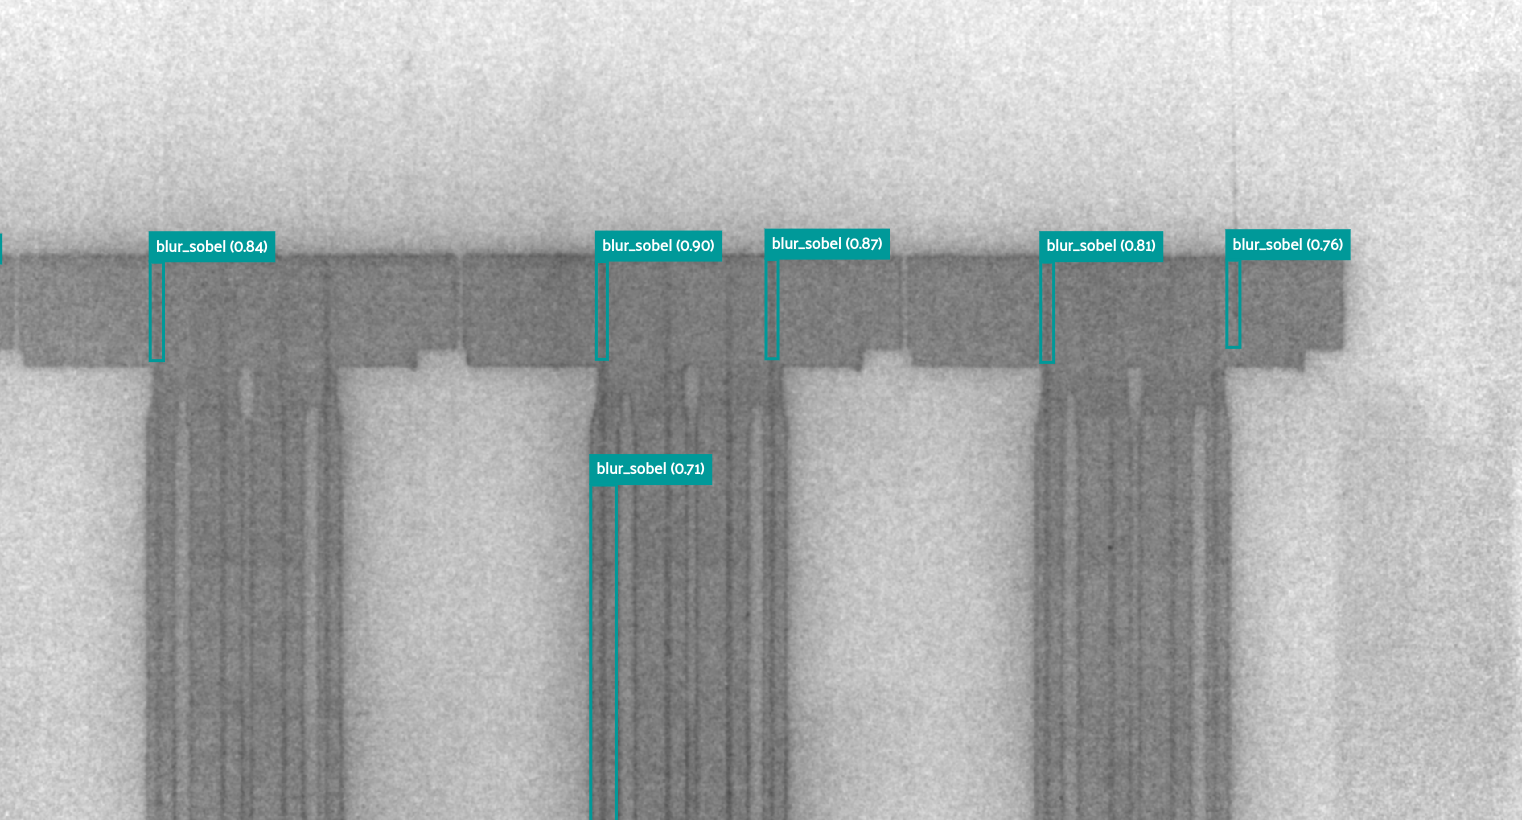
\includegraphics[width=\linewidth]{images/implementation/results/bm/bm_sobel}
    \caption{Using a bitmask and it's sobel filtered version}
  \end{subfigure}

  \begin{subfigure}{.9\textwidth}
    \centering
    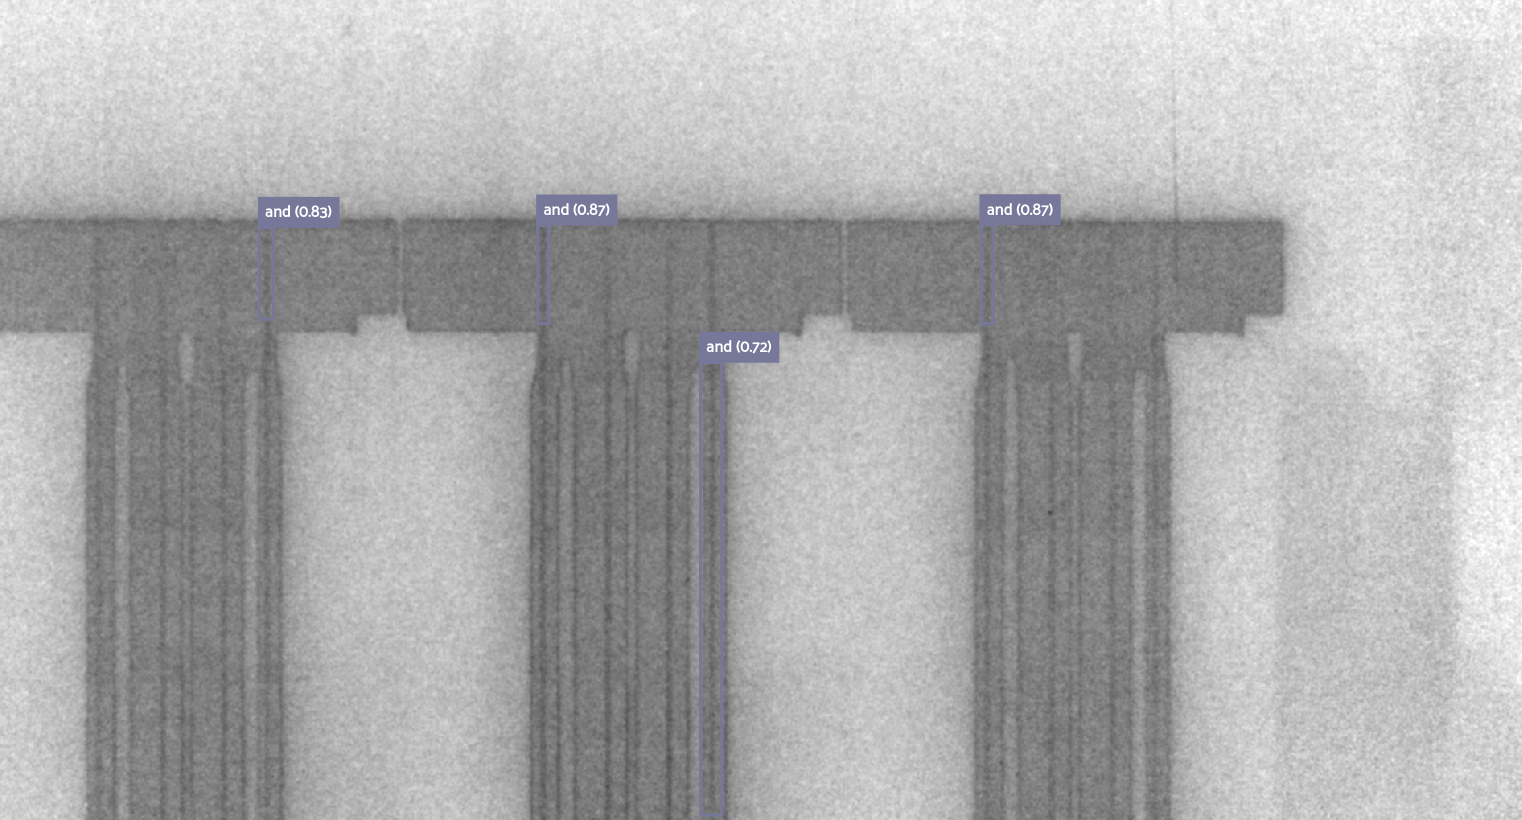
\includegraphics[width=\linewidth]{images/implementation/results/bm/and}
    \caption{Using current and a logical and between the image and the bitmask.}
  \end{subfigure}

  \caption{More alternative bitmask integration methods.}
  \label{app:bm_compare_ext}
\end{figure}
